\documentclass[12pt]{article}

\usepackage[dvips,letterpaper,margin=0.75in,bottom=0.5in]{geometry}
\usepackage{cite}
\usepackage{slashed}
\usepackage{graphicx}
\usepackage{amsmath}
\usepackage{amssymb}
\usepackage{braket}
\usepackage{feynman}
%\usepackage[american,fulldiode]{circuitikz}

\begin{document}
\newcommand{\ihbar}{\ensuremath{i \hbar}}
\newcommand{\dPsidt}{\ensuremath{ \frac{\partial \Psi}{\partial t} }}
\newcommand{\dPsidx}{\ensuremath{ \frac{\partial \Psi}{\partial x} }}
\newcommand{\ddPsidx}{\ensuremath{ \frac{\partial^2 \Psi}{\partial x^2} }}
\newcommand{\dPssdt}{\ensuremath{ \frac{\partial \Psi^*}{\partial t} }}
\newcommand{\dPssdx}{\ensuremath{ \frac{\partial \Psi^*}{\partial x} }}
\newcommand{\ddPssdx}{\ensuremath{ \frac{\partial^2 \Psi^*}{\partial x^2} }}

\newcommand{\dphidt}{\ensuremath{ \frac{d \phi}{dt} }}
\newcommand{\dpsidx}{\ensuremath{ \frac{d \psi}{dx} }}
\newcommand{\ddpsidx}{\ensuremath{ \frac{d^2 \psi}{dx^2} }}


\date{\vspace{-5ex}}

\title{Name: \line(1,0){275}\\ 
ID: \line(1,0){275}\\
130A - Practice Final}
\date{}

\maketitle

\noindent
{\bf Reminder:} For a $1 + 2 \to 3 + 4$ processes:
\begin{center}
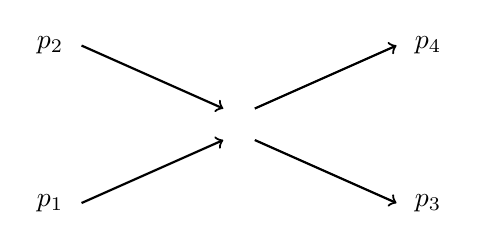
\begin{tikzpicture}[scale=2]
\draw [thick, ->] (0,1) to (0.9,0.6);
\draw [thick, ->] (0,0) to (0.9,0.4);
\draw [thick, ->] (1.1,0.6) to (2,1);
\draw [thick, ->] (1.1,0.4) to (2,0);
\node at (-0.2, 0) {$p_1$};
\node at (-0.2, 1) {$p_2$};
\node at (2.2, 0) {$p_3$};
\node at (2.2, 1) {$p_4$};
\end{tikzpicture}
\end{center}
the Mandelstam variables are:
\begin{eqnarray*}
s &=& (p_1 + p_2)^2c^2 \\ 
t &=& (p_1 - p_3)^2c^2 \\ 
u &=& (p_1 - p_4)^2c^2 \\ 
\end{eqnarray*}

\newpage 

\noindent
{\bf Multiple Choice:} Circle the letter for the one correct answer to each prompt below.\\[5pt]

\noindent
{\bf Problem 1:} The $\Delta$ particle with quark content $uuu$ is\\[5pt]
(A) ...an anti-meson with charge +1e\\[5pt]
(B) ...a baryon with charge +2e\\[5pt]
(C) ...an anti-baryon with charge +1e\\[5pt]
(D) ...a meson with charge +2e\\[10pt]


\noindent
{\bf Problem 2:} The decay:
$$\Sigma^0(uds) \to \lambda^0(uds) + \gamma$$    
(A) ...can only only occur as a weak interaction.\\[5pt]
(B) ...violates charge conservation.\\[5pt]
(C) ...violates baryon number conservation.\\[5pt]
(D) ...proceeds via the electromagnetic interaction.\\[10pt]

\noindent
{\bf Problem 3:} The decay:
$$\Omega^{-}(2252~{\rm MeV}) \to \Xi^{0}(1530~{\rm MeV}) + K^{-}(494~{\rm MeV})$$    
(A) ...violates conservation of energy, because:
$$2252~\rm MeV > 1530~{\rm MeV} + 494~{\rm MeV}$$
(B) ...is a kinematically allowed process.\\[10pt]

\newpage
\noindent
{\bf Problem 4:} The process below, which includes up quarks ($u$) and photons ($\gamma$),
\begin{center}
\begin{feynman}
  \fermion{0.0, 0.0}{1.0, 0.0}
  \fermion{1.0, 0.0}{1.0, 1.0}
  \fermion{1.0, 1.0}{0.0, 1.0}
  \electroweak{1.00, 0.0}{2.00, 0.00}
  \electroweak{1.00, 1.0}{2.00, 1.00}
  \node at (0.5,0.2) {$u$};
  \node at (0.5,0.8) {$u$};
  \node at (1.2,0.5) {$u$};
  \node at (1.5,0.2) {$\gamma$};
  \node at (1.5,0.8) {$\gamma$};
\end{feynman}
\end{center}
(A) ...is a strong interaction due to the exchange of a virtual quarks.\\[5pt]
(B) ...is an electromagnetic interaction due to the presence of virtual photons.\\[5pt]
(C) ...is kinematically forbidden, as the outgoing particles are massless.\\[5pt]
(D) ...shows how the neutral pion ($\pi^0$) can decay to two photons via the electromagnetic interaction.\\[10pt]

\noindent
{\bf Problem 5:} The process shown in the following diagram:
\begin{center}
\begin{feynman}
  \fermion{0.0, 1.0}{1.0, 0.5}
  \fermion{1.0, 0.5}{0.0, 0.0}
  \electroweak{1.00, 0.5}{2.00, 0.5}
  \fermion{3.0, 0.0}{2.0, 0.5}
  \fermion{2.0, 0.5}{3.0, 1.0}
  \node at (0.7,0.2) {$u$};
  \node at (0.7,0.8) {$u$};
  \node at (1.5,0.7) {$\gamma$};
  \node at (2.3,0.2) {$e$};
  \node at (2.3,0.8) {$e$};
\end{feynman}
\end{center}
(A) ...is an $s$-channel process.\\[5pt]
(B) ...is a $t$-channel or $u$-channel process.\\[5pt]
(C) ...is a weak interaction.\\[5pt]
(D) ...does not include any virtual particles.\\[10pt]

\noindent
{\bf Problem 6:} In the lab frame, particles $A$ and $B$ have energies $E_A$ and $E_B$, with momentum $\vec{p}_A$ and $\vec{p}_B$.  What is the $\beta$ of their CMS, as measured in the lab frame?\\[5pt]
(A) $\displaystyle \frac{|\vec{p}_A + \vec{p}_B|}{E_A + E_B}$\\[6pt]
(B) $\displaystyle \frac{E_A + E_B}{|\vec{p}_A + \vec{p}_B|}$\\[6pt]
(C) $\displaystyle \frac{|\vec{p}_A|}{E_A}+\frac{|\vec{p}_B|}{E_B}$\\[6pt]
(D) $\displaystyle \frac{E_A}{|\vec{p}_A|}+\frac{E_B}{|\vec{p}_B|}$\\[10pt]

\newpage

\noindent
{\bf Problem 7:} In the lab frame, a particle with mass $M$ decays into two particles $A$ and $B$.  The four-momentum of particle $A$ is $p_A$, and the four-momentum of particle $B$ is $p_B$.  The quantity $(p_A + p_B)^2$:\\[5pt]
(A) ...depends on the reference frame.\\[5pt]
(B) ...is equal to zero.\\[5pt]
(C) ...depends on the angle $\theta$ between between $\vec{p}_A$ and $\vec{p}_B$.\\[5pt]
(D) ...is equal to $(Mc)^2$\\[10pt]

\noindent
{\bf Problem 8:} The fundamental property of the gamma matrices:\\[5pt]
$$\{ \gamma^u, \gamma^w\} = 2 g^{uw}$$\\[5pt]
(A) ...ensures that $(\gamma^0)^2 = (\gamma^1)^2 = (\gamma^2)^2 = (\gamma^3)^2 = 1$\\[5pt]
(B) ...implies that $\gamma^0\gamma^1\gamma^2 = \gamma^3$\\[5pt]
(C) ...ensures that they transform as $\widetilde{\gamma}^u = \Lambda^u_w \gamma^w$ where $\Lambda$ is a Lorentz transformation.\\[5pt]
(D) ...implies that $\gamma^0\gamma^1 = -\gamma^1\gamma^0$\\[10pt]

\noindent
{\bf Problem 9:} For scattering of a hard sphere, the differential cross-section is:
$$\frac{d\sigma}{d\Omega} = \frac{R^2}{4}$$
The total cross section is therefore:\\[8pt]
(A) $\displaystyle \frac{R^2}{4}$\\[6pt]
(B) $\pi R^2$\\[5pt]
(C) $2\pi R$\\[5pt]
(D) $0$\\[10pt]


\noindent
{\bf Problem 10:} Which of the following is {\bf not} a relativistic invariant:\\[5pt]
(A) $\overline{\psi}\psi$\\[5pt]
(B) $p^u q_u$ for four vectors $p$ and $q$.\\[5pt]
(C) $\psi^\dagger \psi$\\[5pt]
(D) $\psi^\dagger \gamma^0 \psi$\\[10pt]

\newpage

\noindent
{\bf Longer Problems:} Show all work needed to answer each prompt below.\\[5pt]  

\noindent
{\bf Problem 11:} Consider the following Feynman diagram:\\[5pt]
\begin{center}
\begin{feynman}
  \fermion{0.0, 1.0}{1.0, 0.8}
  \fermion{1.0, 0.8}{2.0, 1.0}
  \electroweak{1.0, 0.8}{1.0, 0.2}
  \fermion{2.0, 0.0}{1.0, 0.2}
  \fermion{1.0, 0.2}{0.0, 0.0}
\end{feynman}
\end{center}
~\\[5pt]
\noindent
(A) Apply labels $e$ and $\mu$ to the diagram so that it describes the QED process
$$e^- + \mu^+ \to e^- + \mu^+$$\\[5pt]
(B) Label the four momentum for each external ($p_i$) and internal ($q_i$) particle.\\[5pt]
(C) When calculating the amplitude following the Feynman rules, over what will you integrate?  (Example, but incorrect, answer:  $d^3p_1$)\\[5pt]
(D) In the last step, you will cancel a delta function for overall conservation of four-momentum.  Write the delta function you should expect to encounter.

\newpage

\noindent
{\bf Problem 12:} An atom, at rest in the lab frame, is in an excited state of mass $M$.  It emits a photon of momentum $q$.  What is the mass of the atom after the emission of the the photon?

\newpage








\end{document}


